\subsection{Baseline}
Establishing a baseline is fundamental for assessing model efficacy in financial time series analysis. The baseline, represented as a horizontal line projecting the last closing price from the training dataset, serves as an essential visionary, positing that the future stock price will remain unchanged \cite{hyndman2018forecasting}. This approach is instrumental in setting a preliminary benchmark, ensuring that advanced models demonstrate superior predictive capabilities over this simplistic assumption \cite{makridakis2020m4}.


\subsection{Quantum Recurrent Neural Networks}
To gain initial insights into addressing the problem of time series forecasting through Quantum Algorithms, we employ a methodology analogous to classical Machine Learning approaches. This Algorithm is subsequently adapted for its quantum analog. As elucidated in the preceding background section, leveraging recurrence constitutes a prevalent strategy for simultaneously processing multiple temporal steps \cite{li2023quantum} \cite{bausch2020recurrent}.

Similar to its classical counterpart, the model introduced herein represents a fundamental implementation within the realm of Quantum models. In the context of this paper, its primary purpose is to facilitate a comprehensive exploration of quantum models employing recurrence, while concurrently offering a substantive basis for comparison with our ultimate implementation.

The implemented QRNN utilizes recurrent cells composed of three distinct components: Data Encoding, the chosen Ansatz, and quantum measurement to yield an output.

In the Data Encoding phase, we adopt Angle Encoding as our encoding layer to ensure comparability and mitigate potential drawbacks inherent in this process and moreover to employ a standard and broadly used procedure. Angle Encoding involves representing input data as rotation angles of individual qubits \cite{li2023quantum}.

The primary objective of the Ansatz is to establish entanglement among the qubits within the circuit. To achieve this, we employ an Ansatz that creates entanglement through two-qubit gates, as detailed in \cite{Kraus_2001}. The complete Ansatz utilized in this study is depicted in Figure ~\ref{fig:qrnn-ansatz}.

Similar to the data encoding strategy, the quantum measurement process aims for comparability with other quantum neural networks. Hence, we opt for a widely acknowledged and standard method of qubit measurement. The Pauli-Z measurement emerges as the most straightforward approach, determining whether an individual qubit is in the state of $\ket{0}$ or $\ket{1}$, as discussed in \cite{li2023quantum}.

The finalized QRNN-Cell is illustrated in Figure ~\ref{fig:vqc}. As previously elucidated, the last missing step is to stack the cells in a repetitive manner, culminating in the completion of the QRNN model \cite{bausch2020recurrent}.

\begin{figure}[!htbp]
\centering
\scalebox{0.45}{
\begin{quantikz}
 \lstick{\ket{0}} & \qw & \gate{RX(\theta^{1}_{1})} & \gate{RZ(\theta^{2}_{1})} & \gate{RX(\theta^{3}_{1})} & \qw & \ctrl{1} & \qw & \ctrl{1} & \qw & \qw & \qw & \qw & \qw & \qw & \targ{} & \gate{\gamma_{4}} & \targ{} & \qw\\
 \lstick{\ket{0}} & \qw & \gate{RX(\theta^{1}_{2})} & \gate{RZ(\theta^{2}_{2})} & \gate{RX(\theta^{3}_{2})} & \qw & \targ{} & \gate{\gamma_{1}} & \targ{} & \ctrl{1} & \qw & \ctrl{1} & \qw & \qw & \qw  & \qw  & \qw  & \qw & \qw\\
 \lstick{\ket{0}} & \qw & \gate{RX(\theta^{1}_{3})} & \gate{RZ(\theta^{2}_{3})} & \gate{RX(\theta^{3}_{3})} & \qw & \qw & \qw & \qw & \targ{} & \gate{\gamma_{2}} & \targ{} & \ctrl{1} & \qw & \ctrl{1} & \qw & \qw & \qw & \qw\\
 \lstick{\ket{0}} & \qw & \gate{RX(\theta^{1}_{4})} & \gate{RZ(\theta^{2}_{4})} & \gate{RX(\theta^{3}_{4})} & \qw & \qw & \qw & \qw & \qw & \qw & \qw & \targ{} & \gate{\gamma_{3}} & \targ{} & \ctrl{-3} & \qw & \ctrl{-3} & \qw
\end{quantikz}
}
\caption{QRNN-Ansatz.}
\label{fig:qrnn-ansatz}
\end{figure}

\subsection{Quantum Long Short-Term Memory}
In this study, we propose an extension of classical LSTM networks into the quantum domain. This extension involves replacing the classical neural networks within the LSTM cells with VQCs. These VQCs serve dual purposes: feature extraction and data compression, aiming to leverage the unique computational advantages of quantum mechanisms \cite{chen2020quantum}.

\begin{figure}[!htbp]
    \centering
    \scalebox{0.38}{
    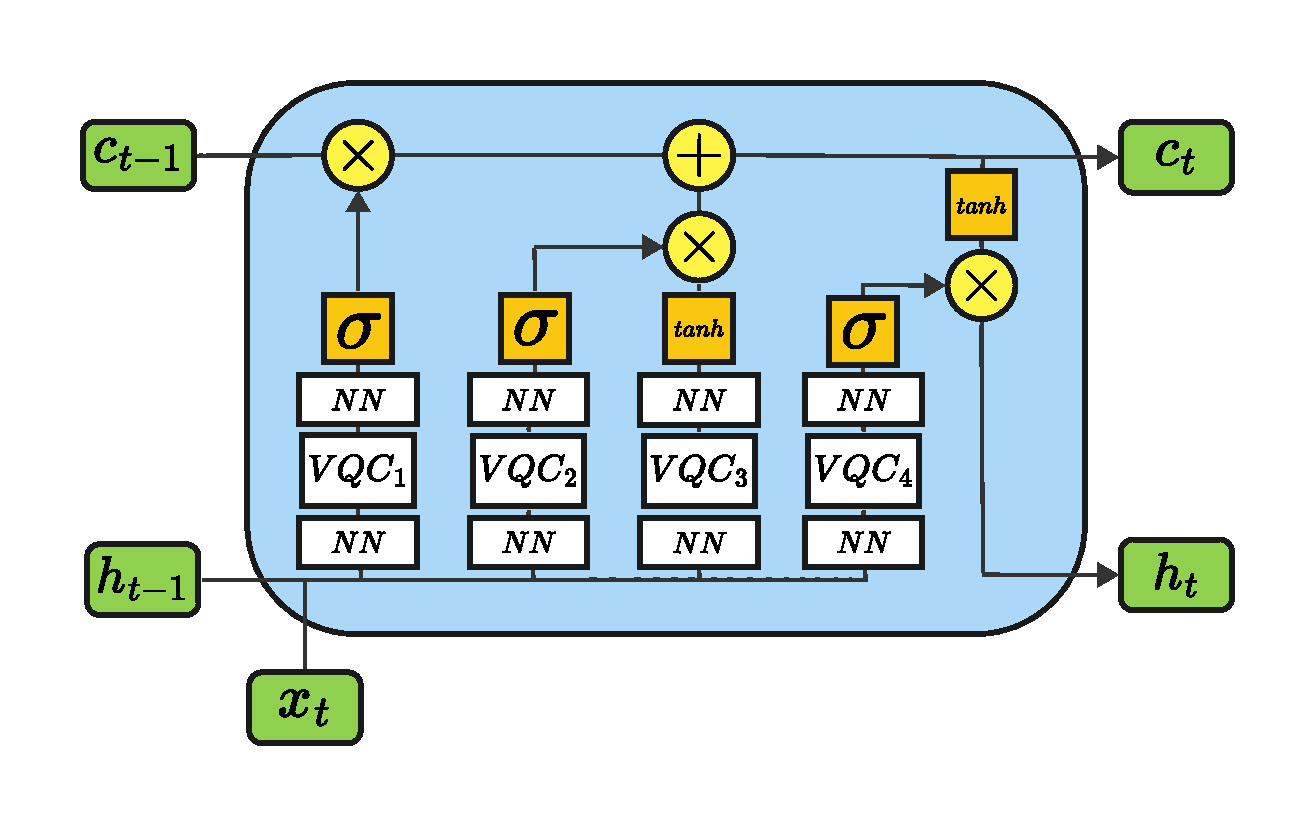
\includegraphics{QCP Report Template/gfx/qlstm.pdf}
    }
    \caption{QLSTM Cell With VQCs and pre- and post-processing NN}
    \label{fig:qlstm}
\end{figure}

The core unit of our proposed QLSTM architecture is the QLSTM cell depicted in \ref{fig:qlstm}, which consists of a stack of VQC blocks. Specifically, a QLSTM cell contains four VQCs. The input to these VQCs is a scaled combination of the previous time step's hidden state \( h_{t-1} \) and the current input vector \( x_t \). This scaling is performed by a classical linear neural network layer, aligning the inputs to the required four-qubit format, which we call $v_t$. The output from each VQC is a four-vector set, representing the Pauli Z expectation values for each qubit. These outputs are subsequently scaled using another classical linear neural network layer to achieve the desired output dimension, as depicted in \ref{fig:qlstm_nn}. In our case, this dimension is 1, representing a predicted stock price. The measured values are then processed through nonlinear activation functions, specifically sigmoid and tanh.

The mathematical formulation of a QLSTM cell is as follows:
\begin{equation}
y_t &= \text{classical NN input layer}(v_t)
\end{equation}
\begin{equation}
\text{forget}_t &= \sigma(\text{classical NN output layer}(VQC_1(y_t)))
\end{equation}
\begin{equation}
\text{input}_t &= \sigma(\text{classical NN output layer}(VQC_2(y_t)))
\end{equation}
\begin{equation}
\text{update}_t &= \tanh(\text{classical NN output layer}(VQC_3(y_t)))
\end{equation}
\begin{equation}
\text{output}_t &= \sigma(\text{classical NN output layer}(VQC_4(y_t)))
\end{equation}
\begin{equation}
c_t &= (f_t \cdot c_{t-1}) + (i_t \cdot g_t)
\end{equation}
\begin{equation}
h_t &= o_t \cdot \tanh(c_t)
\end{equation}

\begin{figure}[!htbp]
    \centering
    \scalebox{0.30}{
    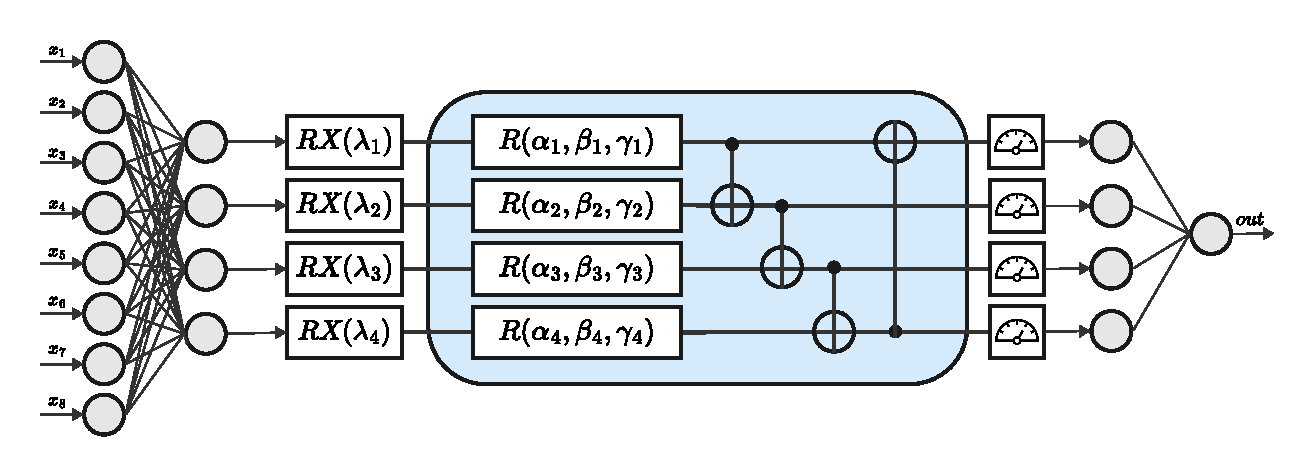
\includegraphics{QCP Report Template/gfx/qlstm_nn.pdf}
    }
    \caption{QLSTM VQC with pre- and post-processing NN}
    \label{fig:qlstm_nn}
\end{figure}
The operation of the QLSTM cell can be divided into three main blocks:

\textbf{Forget Block:} $VQC_1$ processes \( v_t \), outputting a vector \( f_t \) in the range [0,1] via a sigmoid function. This vector determines the extent to which elements in the previous cell state \( c_{t-1} \) are retained or forgotten by element-wise multiplication.

\textbf{Input and Update Block:} This block decides what new information is added to the cell state. $VQC_2$ and $VQC_3$ process \( v_t \), with their outputs determining which values are updated in the cell state. The result from $VQC_2$, after sigmoid activation, is multiplied element-wise by the new candidate cell state \( \tilde{C}_t \), generated by $VQC_3$ after tanh activation, to update the cell state.

\textbf{Output Block:} After updating the cell state, $VQC_4$ processes \( v_t \) and, following sigmoid activation, determines the relevant values in the cell state \( c_t \) for the output. The cell state is then passed through a tanh function and multiplied element-wise by the output from $VQC_4$ to produce the final output or hidden state \( h_t \).


\subsection{Pseudo Code}
\begin{algorithm}[H]
\caption{Training and Testing of the Models}
\begin{algorithmic}[1]
\STATE Initialize the model with its parameters
\STATE Initialize the loss function
\STATE Initialize Adam optimizer
\STATE Initialize train loader with stock data
\STATE Initialize test loader with stock data
\FOR{each epoch}
\FOR{each stock}
\STATE Set model to train mode
\FOR{X\textunderscore Batch, Y\textunderscore Batch in train loader}
\STATE Get model output from X\textunderscore Batch
\STATE Calculate loss from the output and Y\textunderscore Batch
\STATE Use early stopping
\ENDFOR
\STATE Calculate average loss
\STATE Apply linear decay learning rate scheduler
\ENDFOR
\ENDFOR
\STATE Save model
\STATE Set model to evaluation mode
\FOR{X\textunderscore Batch, Y\textunderscore Batch in test loader}
\STATE Get model output from X\textunderscore Batch
\STATE Calculate trend accuracy from the output and Y\textunderscore Batch
\ENDFOR
\STATE Calculate average test loss

\end{algorithmic}
\end{algorithm}